
\documentclass{beamer}
\usecolortheme{dove}
\setbeamertemplate{navigation symbols}{}
\usepackage{amsmath,amssymb,amsfonts,amsthm, multicol, subfigure, color}
\usepackage{bm}
\usepackage{graphicx}
\usepackage{tabularx}
\usepackage{booktabs}
\usepackage{hyperref}
\usepackage{pdfpages}
\usepackage{xcolor}
\definecolor{seagreen}{RGB}{46, 139, 87}
\def\independenT#1#2{\mathrel{\rlap{$#1#2$}\mkern2mu{#1#2}}}
\newcommand\indep{\protect\mathpalette{\protect\independenT}{\perp}}
\def\log{\text{log}}
\newcommand\logit{\text{logit}}
\newcommand\iid{\stackrel{\text{iid}}{\sim}}
\newcommand\E{\text{E}}
\newcommand\V{\text{V}}
\renewcommand\P{\text{P}}
\newcommand{\Cov}{\text{Cov}}
\newcommand{\Cor}{\text{Cor}}
\newcommand\doop{\text{do}}
\usepackage{stackrel}
\usepackage{tikz}
\usetikzlibrary{arrows,shapes.arrows,positioning,shapes,patterns,calc}
\newcommand\slideref[1]{\vskip .1cm \tiny \textcolor{gray}{{#1}}}
\newcommand\red[1]{\color{red}#1}
\newcommand\blue[1]{\color{blue}#1}
\newcommand\gray[1]{\color{gray}#1}
\newcommand\seagreen[1]{\color{seagreen}#1}
\newcommand\purple[1]{\color{purple}#1}
\newcommand\orange[1]{\color{orange}#1}
\newcommand\black[1]{\color{black}#1}
\newcommand\white[1]{\color{white}#1}
\newcommand\teal[1]{\color{teal}#1}
\newcommand\magenta[1]{\color{magenta}#1}
\newcommand\Fuchsia[1]{\color{Fuchsia}#1}
\newcommand\BlueGreen[1]{\color{BlueGreen}#1}
\newcommand\bblue[1]{\textcolor{blue}{\textbf{#1}}}
\newcommand\bred[1]{\textcolor{red}{\textbf{#1}}}
\newcommand\bgray[1]{\textcolor{gray}{\textbf{#1}}}
\newcommand\bgreen[1]{\textcolor{seagreen}{\textbf{#1}}}
\newcommand\bref[2]{\href{#1}{\color{blue}{#2}}}
\colorlet{lightgray}{gray!40}
\pgfdeclarelayer{bg}    % declare background layer for tikz
\pgfsetlayers{bg,main} % order layers for tikz
\newcommand\mycite[1]{\begin{scriptsize}\textcolor{darkgray}{(#1)}\end{scriptsize}}
\newcommand{\tcframe}{\frame{
%\small{
\only<1|handout:0>{\tableofcontents}
\only<2|handout:1>{\tableofcontents[currentsection]}}
%}
}

\usepackage[round]{natbib}
\bibliographystyle{humannat-mod}
\setbeamertemplate{enumerate items}[default]
\usepackage{mathtools}

\newcommand{\goalsframe}{\begin{frame}{Learning goals for today}
At the end of class, you will be able to:
\begin{enumerate}
\item Make causal claims under only highly credible assumptions*
\end{enumerate} \vskip .2in
*You will not get a point estimate.\\You will get an interval.\\It might be a very wide interval.
\end{frame}}

\newcommand{\goalsframepause}{\begin{frame}{Learning goals for today}
At the end of class, you will be able to:
\begin{enumerate}
\item Make causal claims under only highly credible assumptions* \pause
\end{enumerate} \vskip .2in
*You will not get a point estimate.\\You will get an interval.\\It might be a very wide interval.
\end{frame}}

\title{4. Sharp bounds and the limits of assumption-free inference}
\author{Ian Lundberg\\Cornell Info 6751: Causal Inference in Observational Settings\\Fall 2022}
\date{1 Sep 2022}

\begin{document}

\maketitle

\goalsframepause

\begin{frame}
\Large
A running example:\\The effects of mass incarceration
\end{frame}

\begin{frame}{U.S. federal and state prison population\footnote{\tiny Source: \bref{https://www.sentencingproject.org/publications/u-s-prison-population-trends-massive-buildup-and-modest-decline/}{The Sentencing Project.} Estimates use data from the Bureau of Justice Statistics.}}

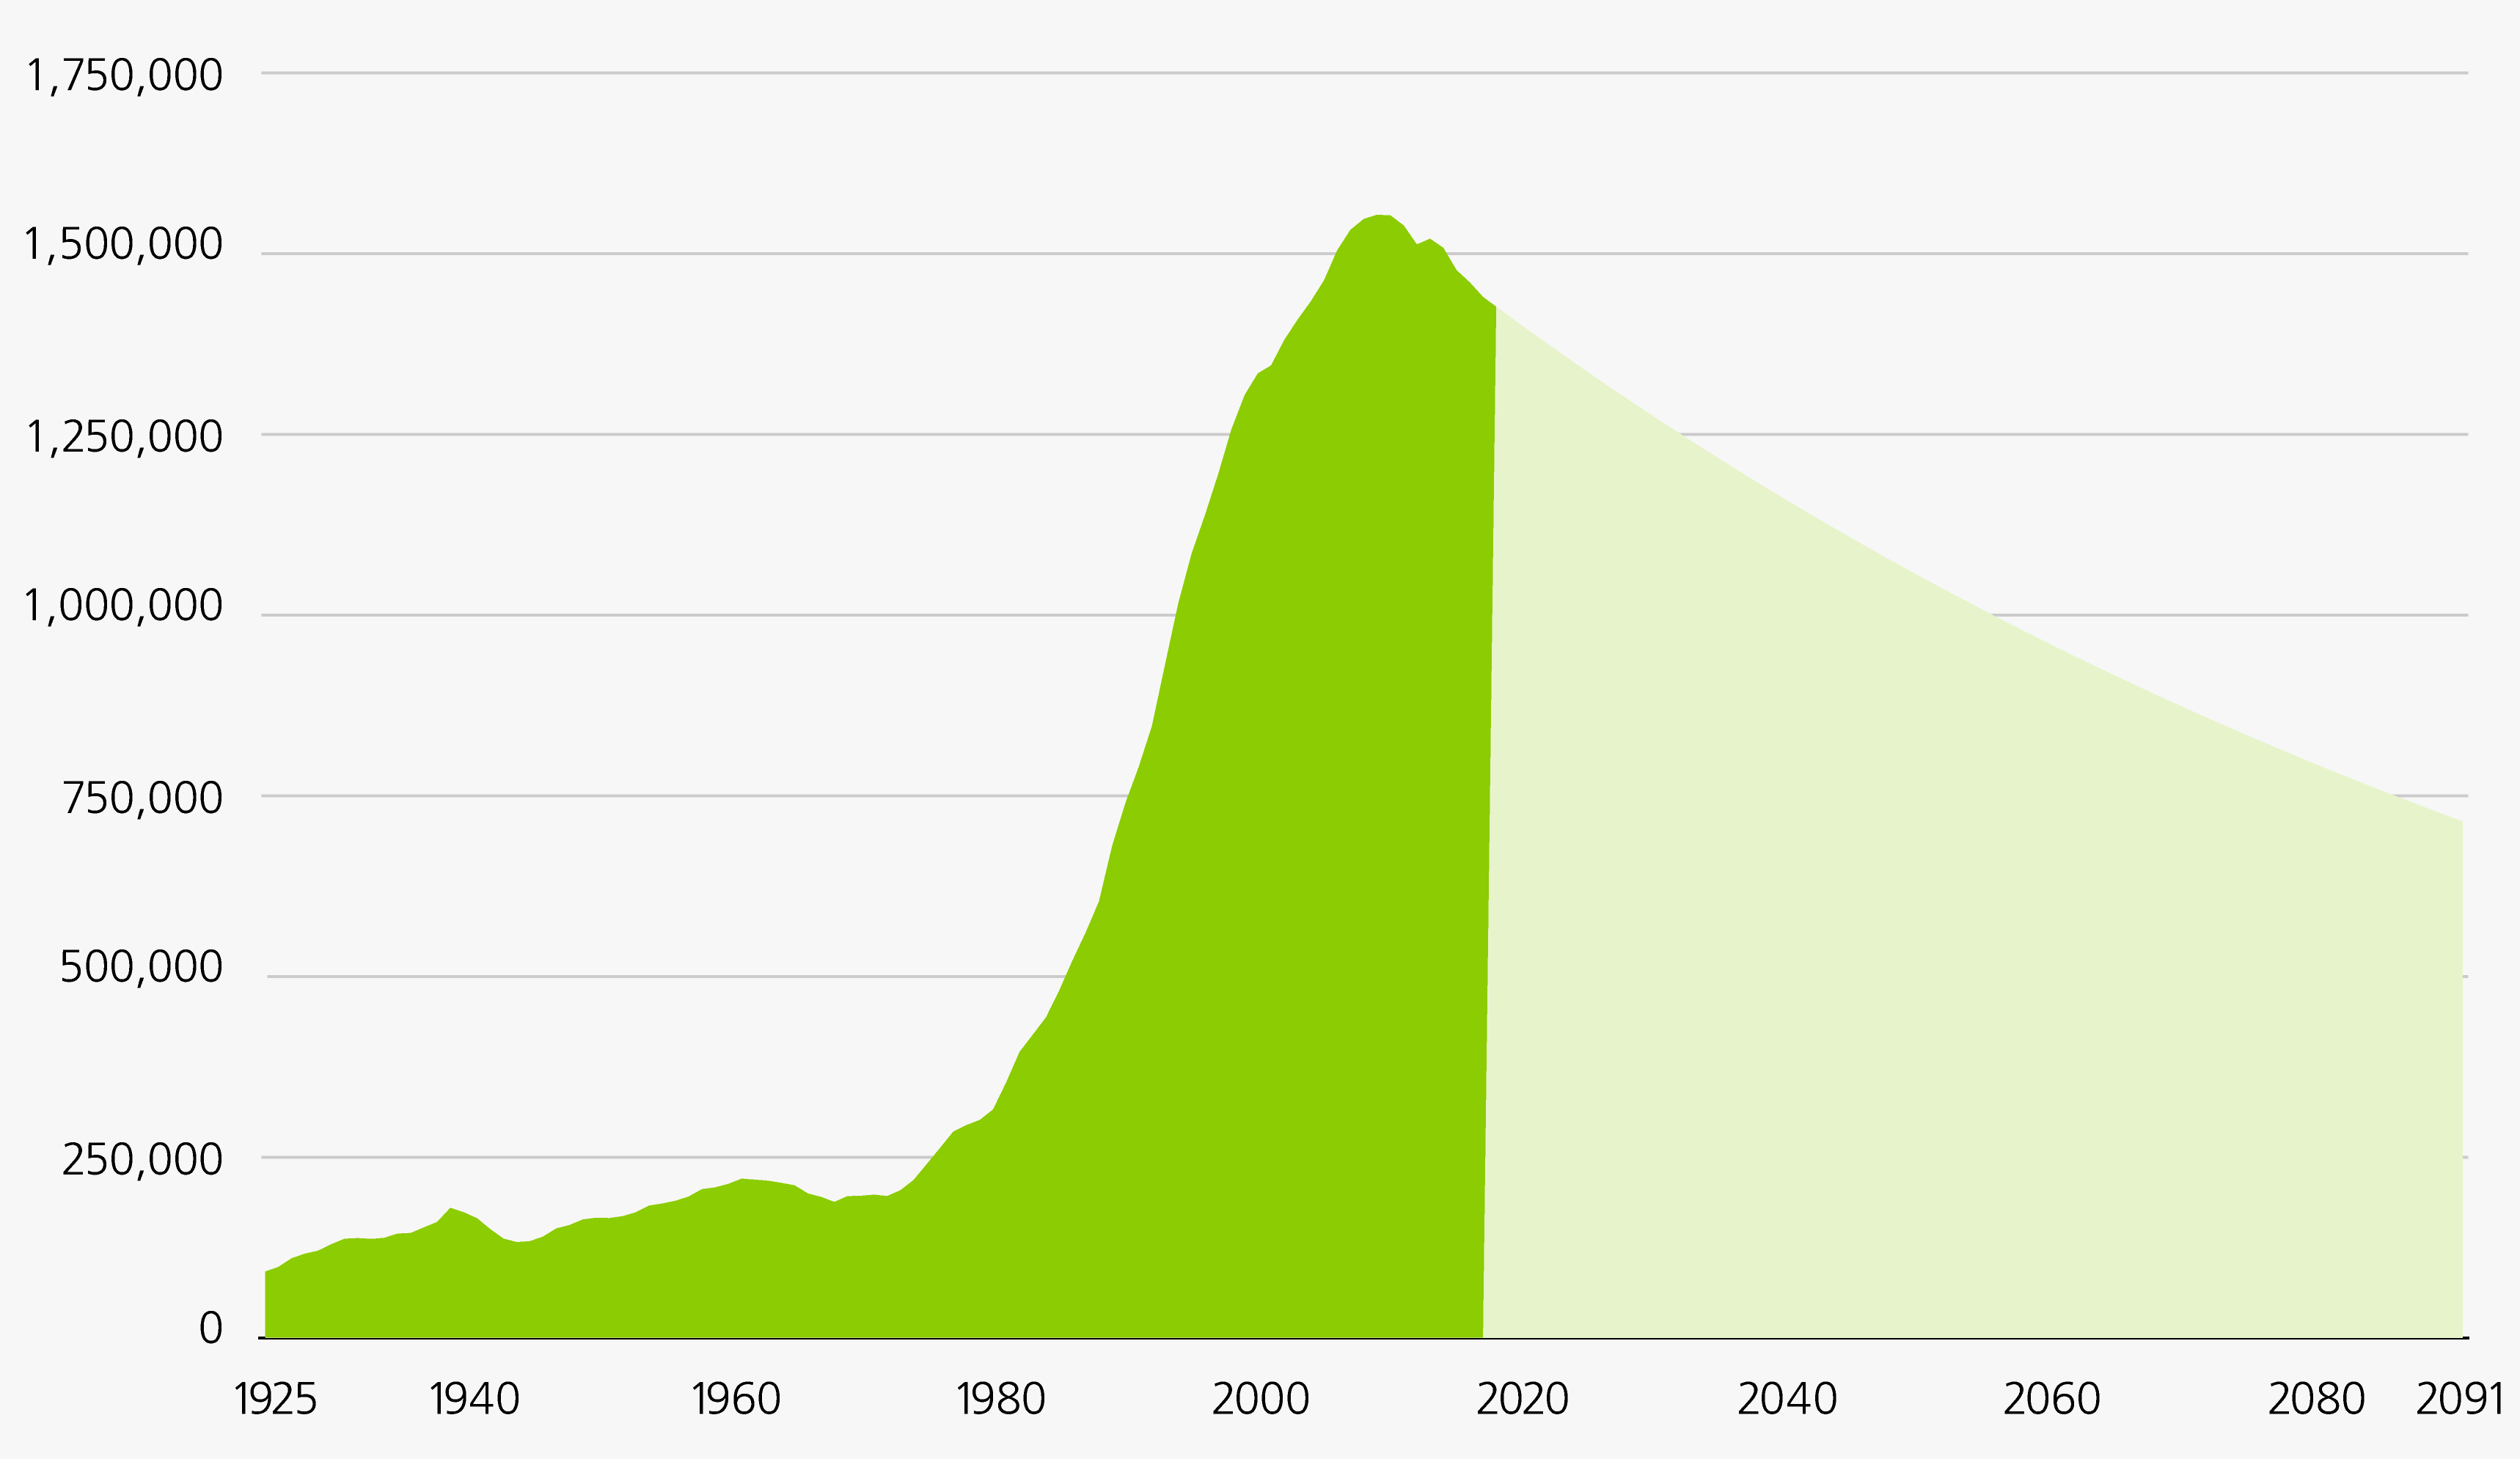
\includegraphics[width = \textwidth]{figures/sentencingProject_trend}

\end{frame}

\begin{frame}

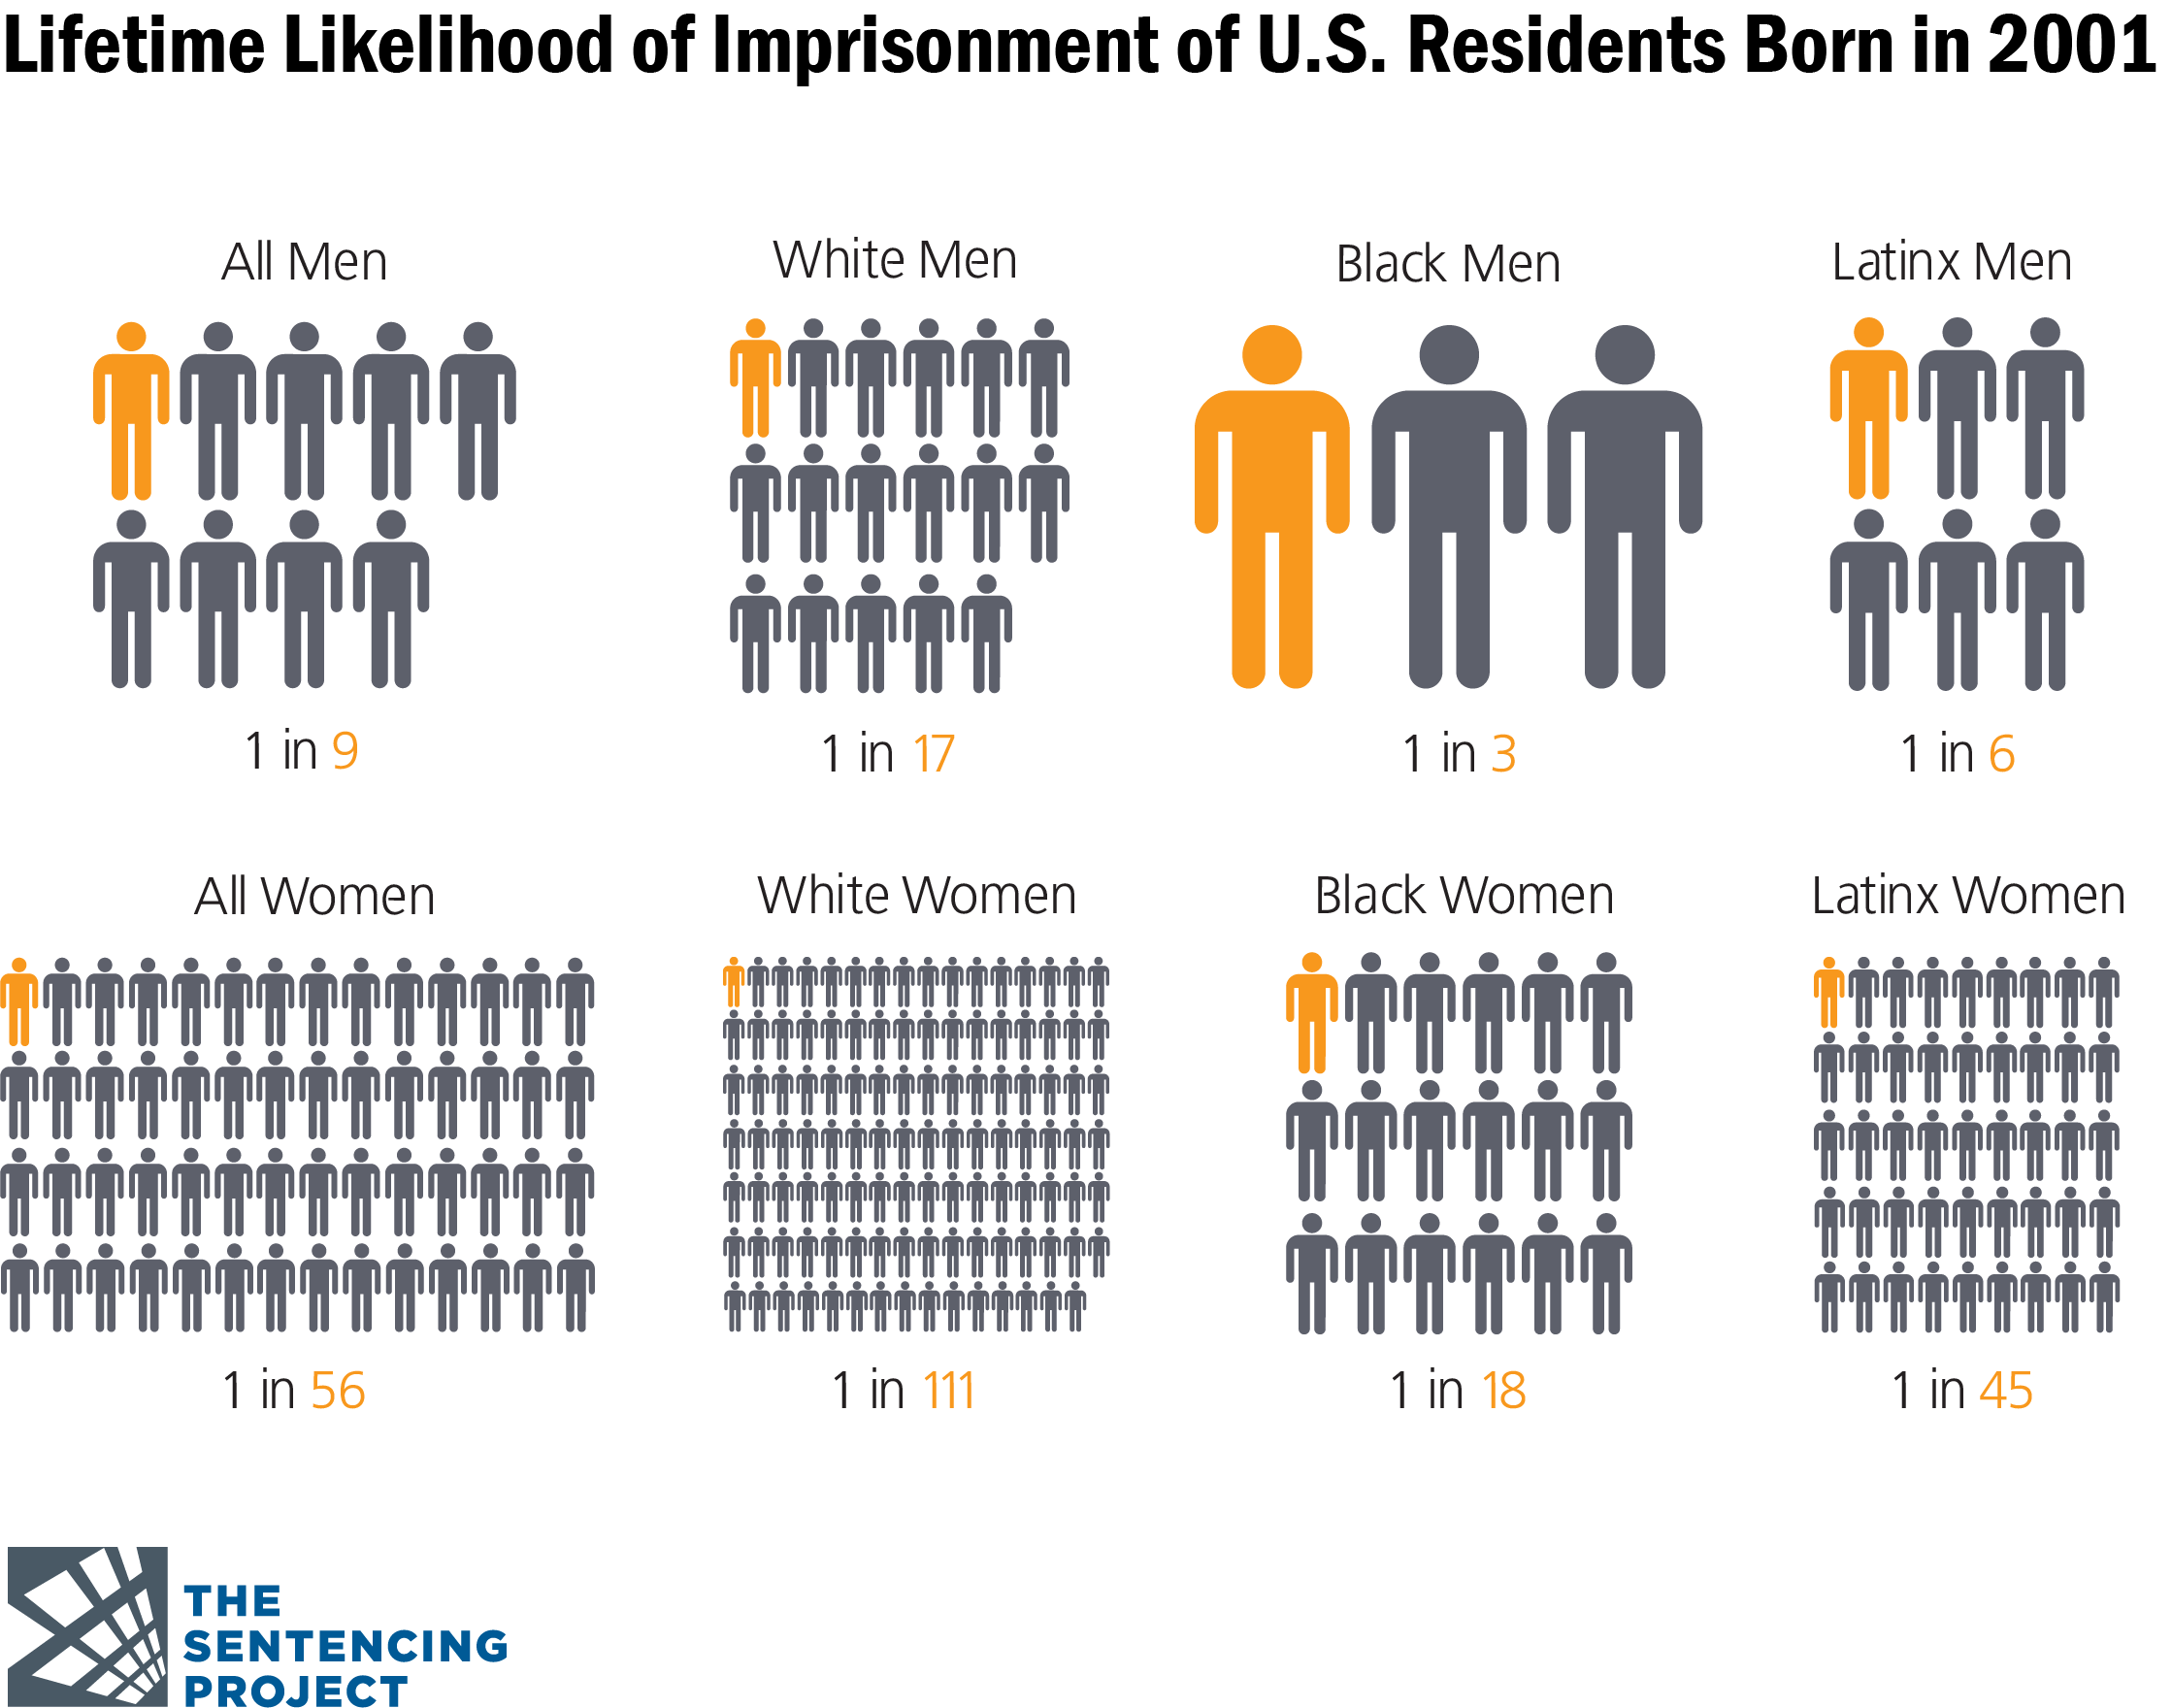
\includegraphics[width = \textwidth]{figures/sentencingProject}\\
{\tiny Source: \bref{https://www.sentencingproject.org/criminal-justice-facts/}{The Sentencing Project.} Life table estimates from 2001 Bureau of Justice Statistics data.}

\end{frame}

\begin{frame}{Running example: Mass incarceration\footnote{Motivation: Western, B. (2006). Punishment and Inequality in America. Russell Sage Foundation.}}
%\pause

Mass incarceration has enormous societal consequences \pause
\begin{itemize}
\item It affects \only<1-4>{{labor market outcomes}}\only<5->{\bblue{labor market outcomes}} \pause
\item It affects family structures \pause
\item It affects neighborhood cohesion
\end{itemize}

\end{frame}

\goalsframe

\begin{frame}{Group exercise}

\huge
\bref{https://docs.google.com/spreadsheets/d/1rKVa7kvfXegvM1-n954grGovYmO6mEbh6jW3BxsKO68/edit?usp=sharing}{[Group Exercise]} \\
\bref{https://docs.google.com/spreadsheets/d/1onsEx7dE2r3kF0uDv_Dvu7qkgY2wY_JMOJ_0Z-F2bMo/edit?usp=sharing}{[Solutions]}

\end{frame}

\goalsframe

\begin{frame}{Let me know what you are thinking}

\begin{huge} \bref{https://tinyurl.com/CausalQuestions}{tinyurl.com/CausalQuestions} \end{huge}
\vskip .7in

Office hours TTh 11am-12pm and at \bref{https://calendly.com/ianlundberg/office-hours}{calendly.com/ianlundberg/office-hours}\\Come say hi!

\end{frame}

\end{document}




